\section{Data Modelling}
	\subsection{CRISP-DM}
	\label{sec:datamodeling}
	\begin{figure}[h]
		\centering
		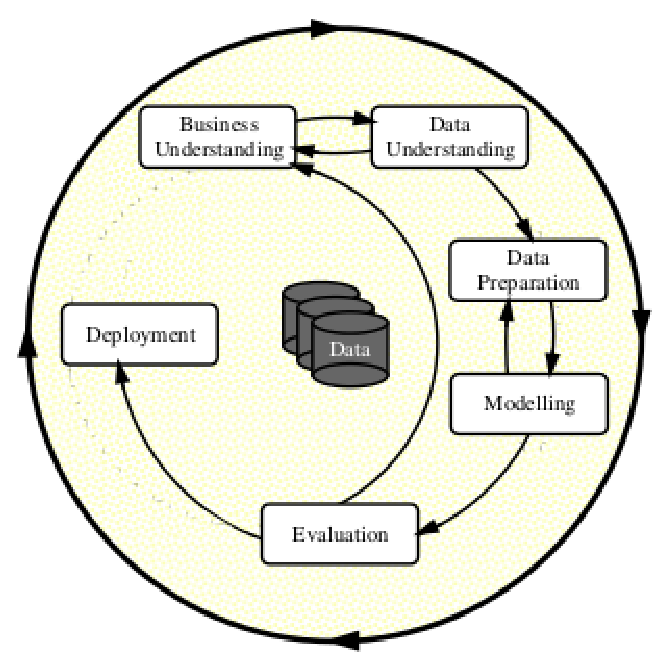
\includegraphics[scale=0.75]{crispdm.eps}
					
		\caption{CRISP-DM\cite{wirth2000crisp} cycle}
		\label{fig:crispdm}

	\end{figure}
	Cross Industry Standard Process for Data Mining\cite{wirth2000crisp} is invented out of necessity for better planning, documentation and communication for Data Mining projects. It's divided in multiple phases, as seen in Figure~\ref{fig:crispdm}. The business understanding phase is to describe the urge and the goal of the project, see Section~\ref{seq:motivation}. The data understanding phase is to learn about the data, what is the source and how it is computed. In Section~\ref{sec:sensorsystems},~\ref{sec:datadescription} and ~\ref{sec:bvsb} the sensors systems are described, how they are used and what the data is. Normally the data is already collected, but this project needs another phase. The data collection phase is described in Section~\ref{sec:datacollection}. The next phase is the data preparation phase. In this project it exists out of two parts. The first part is about preprocessing to compute the dataset, as seen in Section~\ref{sec:preprocessing}. The dataset can be used by the Liacs Data Mining Group for further research. The second part is the feature extraction section, which describes the computing of the training set, seen in Section~\ref{sec:feature}. 
	A model is a generalised representation of the data. An algorithm tries to make relations between attributes. There are three reason to make such an model:
	\begin{enumerate}
		\item Prediction. Predict if a customer is creditworthiness 
		\item Insight. To understand the working and the relations between attributes better. Beer and diapers should be closer together in the supermarket.
		\item Classification. Iris, type of flower. The attributes are known, but experts are needed to classify the flower. A model can also predict the classification.
	\end{enumerate}
	Models needs to be trained, by a training set. The bigger the training set, the better the model, because of chance is higher the set will represent all possible data. The better the model, the better the relations between the attributes are expressed. Next subsection explains how to make a model. When the model is made it's time to analyze the results. Is it possible to achieve the goal? The deployment is the implementation to achieve the goal. This could be a new piece of software for bank employees or a new price for a product. 

	\subsection{WeKa}
	- What is WeKa. java implementation for a lot of data mining algorithms.
	- M5p, Quinlan's M5
	- linear regression
	- neural network
	- results 

	\iffalse

	Business understanding: formulate a goal, what to improve, section 1.2 / 1.3
	Data understanding, What are the systems measuring : Section 2.
	Normally data is already collected, in this project not. So an extra step.
	Data preparation is getting from the raw data to the training set, but in this project there are to steps to produce it.
	First from the raw to the dataset. This dataset can is provided and can be used by the liacs data mining group.
	from dataset to trainingset, in feature extractin section



	Derivate a dataset, use WeKa for modeling, find patterns.

	
	model, A way to describe the data. Generalization.
	prediction, classification, understanding the model.
	- linear regression
	- nearal network
	Now the modeling part.

	Next is the evaluation, which conclusions could be made.

	At least the deployment, implementation of the conclusions. To reach the goal and improvement. 
	\fi
